% 第4章第3节：张量的表示（多维数组、轴、阶、形状、切片）、张量的运算（轴置换、形状重整与向量化、张量积、Kronecker积、张量缩约）、张量运算的性质（重排的性质、张量积的性质、Kronecker积的性质、缩约的性质、各种乘积的形状）。

\section{张量}
\label{sec:ls-tensors-objects}

一批图像要记录样本、通道和两个像素坐标，一批文本要记录样本、位置和特征维度：定位其中一个数需要三个甚至更多的索引，一张二维数表装不下。程序里常把这样的数组换轴、拉平或改变形状，这样做以后哪些量不变？两个向量的全部两两乘积怎样组织，两个矩阵分别作用在不同的轴上时怎样合写，一个多轴数组又怎样沿指定的轴汇总成低阶数组？本节先给出多维数组的记法，再逐一定义轴置换、形状重整、张量积、Kronecker积与缩约，最后按运算整理它们的性质，并说明前两节的内积、矩阵乘法与迹都是缩约的特例。

\subsection{张量的表示}
\label{sec:ls-tensor-representation}

向量用一个索引定位一个数，矩阵用两个。当一个量由多路索引共同决定时，需要更多索引。机器学习中常把这样的多索引数值数组称为\term{张量}（tensor）。
\begin{definition}[多维数值数组]
\label{def:linear-algebra-multidimensional-array}
给定正整数$n_1,\ldots,n_k$，形状为$n_1\times\cdots\times n_k$的数值数组，是从$\{1,\ldots,n_1\}\times\cdots\times\{1,\ldots,n_k\}$到$\mathbb R$的映射。第$j$个索引称为第$j$个\term{轴}（axis），轴数$k$称为数组的\term{阶}（order）。
\end{definition}
按这一说法，向量、矩阵分别是一阶、二阶数组，并约定单个标量是零阶数组。阶是索引的个数，形状记录各轴的长度；单个轴的长度不是阶，$\mathbb R^{100}$中的向量仍是一阶数组。

例如$\bm X\in\mathbb R^{b\times\ell\times d}$可以记录$b$个样本、每个样本$\ell$个位置、每个位置$d$个特征，$x_{i,j,k}$由三个索引共同定位。固定部分索引得到切片：$\bm X_{i,:,:}$保留第$i$个样本，是一个$\ell\times d$矩阵；$\bm X_{i,j,:}$再固定位置，是一个$d$维向量。图~\ref{fig:ls-scalar-vector-matrix-tensor}按“定位一个数需要几个索引”把四类数组并排比较。
\begin{figure}[!htb]
  \centering
  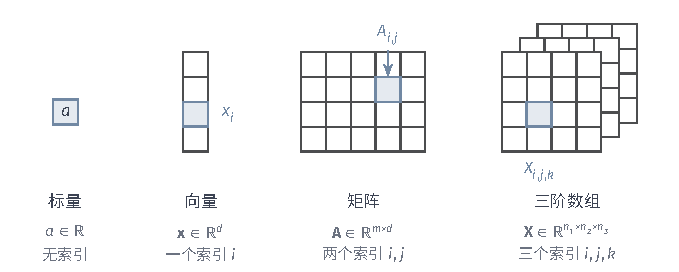
\includegraphics[width=112mm]{figures/00-shared/mathematical-preliminaries-upper/02-linear-spaces/tikz/comprehension-additions/scalar-vector-matrix-tensor.pdf}
  \caption{标量、向量、矩阵与三阶数组的区别。每个面板用蓝色标出一个数：标量本身就是这个数，向量用一个索引$i$定位，矩阵用行列两个索引$i,j$定位，三阶数组再加一个索引$k$选择切片。索引个数称为阶，各轴长度组成形状。}
  \label{fig:ls-scalar-vector-matrix-tensor}
\end{figure}

两个同形数组按位置逐项相加、数乘，规则与向量、矩阵完全相同；两个数组能否相加，仍要求形状相同、对应轴的含义相同。使用多维数组时，须先说清每条轴记录什么：同一个$b\times\ell\times d$数组，若把第二、三轴的含义弄反，后续的每一次汇总都会汇总错的轴。

\subsection{张量的运算}
\label{sec:ls-tensor-operations}

多轴数组的运算按对轴的作用分成三类。轴置换与形状重整只改变元素记录在哪条轴、哪个位置上，不改变数值，也不求和。张量积和它的矩阵形式Kronecker积把多个因子的轴全部保留下来，组合成轴更多的数组。缩约则反过来，指定一对或几对轴对齐相乘后求和，把数组汇总成更低阶的数组。

\subsubsection{轴置换}
\label{sec:ls-tensor-reshaping}
\phantomsection
\label{sec:linear-algebra-tensors-structured-operations}

\term{维度重排}（permutation of axes）按给定顺序调换轴的位置，元素跟随自己的索引移动。计算时先写出新旧索引的对应，再按对应搬运元素。例如把$\bm X\in\mathbb R^{b\times\ell\times d}$的第二、三轴互换，得到$\bm Y\in\mathbb R^{b\times d\times\ell}$，
\[
 y_{i,k,j}=x_{i,j,k}.
\]
第一个轴保持原位，每个样本的切片被转置：$\bm Y_{i,:,:}=(\bm X_{i,:,:})^\top$。下面取一个具体的小数组。
\begin{example}[交换后两条轴]
\label{ex:ls-axis-swap}
给定：$b=1$、$\ell=2$、$d=3$，唯一的样本切片为$\bm X_{1,:,:}=\left[\begin{smallmatrix}1&2&3\\4&5&6\end{smallmatrix}\right]$。
计算：按$y_{1,k,j}=x_{1,j,k}$搬运元素，例如$y_{1,3,2}=x_{1,2,3}=6$，得到
\[
 \bm Y_{1,:,:}=\begin{bmatrix}1&4\\2&5\\3&6\end{bmatrix}.
\]
结论：$\bm Y\in\mathbb R^{1\times3\times2}$，它的样本切片正是原切片的转置。
\end{example}
矩阵的转置是两个轴时唯一的非平凡轴置换。轴的含义跟着轴走，不因位置改变而改变：$\bm Y$的第二轴仍是特征，第三轴仍是位置。

\subsubsection{形状重整与向量化}

\term{形状重整}（reshape）先按指定的遍历顺序把全部元素读成一个数列，再把这个数列按同样的顺序装入另一形状；它只要求元素总数相同。计算分两步：读出、装入。下面的例子比较按行重整与转置。
\begin{example}[按行重整与转置的区别]
\label{ex:ls-reshape-vs-transpose}
给定：$\bm A=\left[\begin{smallmatrix}1&2&3\\4&5&6\end{smallmatrix}\right]$，目标形状为$3\times2$。
计算：按行读出得数列$1,2,3,4,5,6$，再按行装入$3\times2$数组，得到
\[
 \bm R=\begin{bmatrix}1&2\\3&4\\5&6\end{bmatrix},
 \qquad\text{而}\qquad
 \bm A^\top=\begin{bmatrix}1&4\\2&5\\3&6\end{bmatrix}.
\]
结论：$\bm R$与$\bm A^\top$形状相同、所含的数相同，排列却不同。
\end{example}
所以重整不能只给目标形状，还要给遍历顺序；形状相同也不能说明完成了轴交换。图~\ref{fig:vol1-add-linear-transpose-reshape}把两种结果并排放置。
\begin{figure}[!htb]
  \centering
  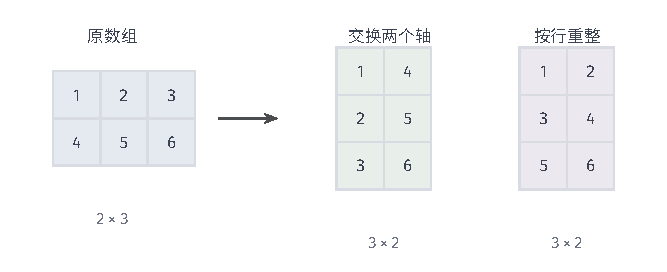
\includegraphics[width=112mm]{figures/00-shared/mathematical-preliminaries-upper/02-linear-spaces/tikz/comprehension-additions/linear-transpose-reshape.pdf}
  \caption{轴交换与按行重整。原数组两行为$(1,2,3)$与$(4,5,6)$；中图转置后两列分别保留原来的两行，右图则把按行读取的数列$1,2,3,4,5,6$依次装入$3\times2$数组。数字及其排列由正文示例直接给出。}
  \label{fig:vol1-add-linear-transpose-reshape}
\end{figure}

形状重整中最常用的一种，是把矩阵按列堆叠成一个长列向量，称为\term{向量化}（vectorization）：
\[
 \operatorname{vec}(\bm A)=(a_{1,1},\ldots,a_{m,1},a_{1,2},\ldots,a_{m,2},\ldots,a_{1,n},\ldots,a_{m,n})^\top,
\]
$m\times n$矩阵的元素$a_{i,j}$位于一维索引$i+(j-1)m$。例如上面的$\bm A$给出$\operatorname{vec}(\bm A)=(1,4,2,5,3,6)^\top$，其中$a_{2,3}=6$位于第$2+(3-1)\cdot2=6$个位置。

多维数组也可以按轴重整成矩阵，称为矩阵展开（unfolding）：把一部分轴合并成行索引，其余轴合并成列索引。例如把$\bm X\in\mathbb R^{b\times\ell\times d}$的前两轴合并为行，得到$b\ell\times d$矩阵，每行是一个样本在一个位置上的特征。选哪些轴合并，决定展开结果的形状，也决定后续乘积汇总哪个轴。

\subsubsection{张量积}
\label{sec:ls-tensor-products}
\phantomsection
\label{sec:linear-algebra-joint-operations}

两个向量的全部两两乘积排成一个数组，就是它们的张量积。设$\bm x\in\mathbb R^m$、$\bm y\in\mathbb R^n$，\term{张量积}（tensor product）$\bm x\otimes\bm y$是$m\times n$数组，
\[
 (\bm x\otimes\bm y)_{i,j}=x_i y_j.
\]
写成矩阵，$\bm x\otimes\bm y=\bm x\bm y^\top$，正是分块乘法式~\eqref{eq:ls-product-outer-sum}中“一列乘一行”的矩阵。每个因子各占结果的一条轴，下面称为一个槽位。三个向量的张量积$(\bm x\otimes\bm y\otimes\bm z)_{i,j,k}=x_i y_j z_k$保留三个槽位，多重张量积按同样规则逐槽位相乘。下面计算两个二维向量的张量积。
\begin{example}[两个二维向量的张量积]
\label{ex:ls-tensor-product-two-vectors}
给定：$\bm x=(1,2)^\top$，$\bm y=(3,-1)^\top$。
计算：
\[
 \bm x\otimes\bm y=\begin{pmatrix}1\cdot3&1\cdot(-1)\\2\cdot3&2\cdot(-1)\end{pmatrix}=\begin{pmatrix}3&-1\\6&-2\end{pmatrix}.
\]
结论：第$i$行是$x_i\bm y^\top$，所以每一行都是$\bm y^\top$的倍数；同理，每一列都是$\bm x$的倍数。
\end{example}
图~\ref{fig:ls-tensor-product-slots}展示张量积怎样保留两个因子的槽位。
\begin{figure}[htbp]
  \centering
  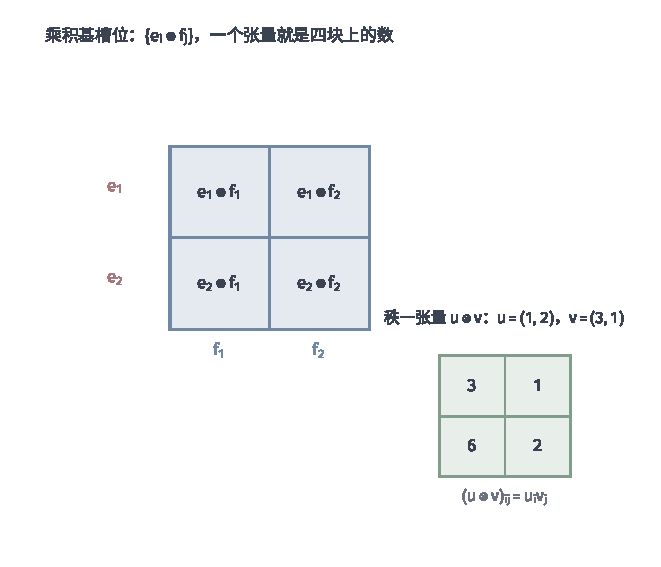
\includegraphics[width=112mm]{figures/00-shared/mathematical-preliminaries-upper/02-linear-spaces/matplotlib/ls-tensor-product-slots/ls-tensor-product-slots.pdf}
  \caption{张量积并排保留两个因子的槽位。左：$\bm u\in\mathbb R^2$、$\bm v\in\mathbb R^3$。右：$\bm u\otimes\bm v$排成$2\times3$网格，每行由$\bm v$方向复制并按$u_i$缩放；它是简单张量，数值由$\bm u=(1,0.6)$、$\bm v=(1,0.5,0.2)$直接相乘得到，是教学构造。}
  \label{fig:ls-tensor-product-slots}
\end{figure}

形如$\bm x\otimes\bm y$的数组称为\term{简单张量}（simple tensor）。由示例~\ref{ex:ls-tensor-product-two-vectors}的结论，简单张量的各行都是同一个向量的倍数。并非每个二阶数组都是简单张量，下面是一个反例。
\begin{example}[反例：单位矩阵不是简单张量]
\label{ex:ls-identity-not-simple}
给定：$\bm I_2$，它的两行为$(1,0)$与$(0,1)$。
验证：若$\bm I_2=\bm x\otimes\bm y$，则两行分别是$x_1\bm y^\top$与$x_2\bm y^\top$。两行都非零，所以$x_1,x_2\neq0$，两行都是$\bm y^\top$的非零倍数，从而彼此成比例。但$(1,0)$与$(0,1)$不成比例。
结论：$\bm I_2$不能写成任何$\bm x\otimes\bm y$，它不是简单张量。
\end{example}
不过，每个$m\times n$数组$\bm T$都是简单张量的和，
\[
 \bm T=\sum_{i,j}t_{i,j}\,\bm e_i\otimes\bm f_j,
\]
其中$\bm e_i$、$\bm f_j$分别是$\mathbb R^m$与$\mathbb R^n$的标准坐标向量，$\bm e_i\otimes\bm f_j$只在位置$(i,j)$为$1$。

张量积的用处，是把同时依赖两组输入的读取化为对单个数组的线性读取。设实值函数$B(\bm x,\bm y)$对$\bm x$、$\bm y$分别保持线性组合（称为双线性）。把$\bm x=\sum_ix_i\bm e_i$、$\bm y=\sum_jy_j\bm f_j$代入，按两次线性展开，
\[
 B(\bm x,\bm y)=\sum_{i,j}x_iy_j\,B(\bm e_i,\bm f_j)=\sum_{i,j}g_{i,j}(\bm x\otimes\bm y)_{i,j}
 =\langle\bm G,\bm x\otimes\bm y\rangle_{\mathrm F},
\]
其中$g_{i,j}=B(\bm e_i,\bm f_j)$。所以双线性读取由一张固定的系数表$\bm G$决定，并且它对数组$\bm x\otimes\bm y$是线性的。以欧氏内积$B(\bm x,\bm y)=\bm x^\top\bm y$（$m=n$）为例，$g_{i,j}=\langle\bm e_i,\bm e_j\rangle$，即$\bm G=\bm I$，读取就是把$\bm x\otimes\bm y$的对角线加起来。

二阶张量与矩阵是同一组数的两种记录：张量强调槽位来自哪一组输入，矩阵强调行列在乘法中的角色。

\subsubsection{Kronecker积}

两个矩阵分别作用在两条轴上时，联合作用可以写成一张大矩阵。对$\bm A\in\mathbb R^{m\times n}$、$\bm B\in\mathbb R^{p\times q}$，定义Kronecker积
\begin{equation}
 \bm A\otimes\bm B
 =\begin{bmatrix}
  A_{1,1}\bm B&\cdots&A_{1,n}\bm B\\
  \vdots&\ddots&\vdots\\
  A_{m,1}\bm B&\cdots&A_{m,n}\bm B
 \end{bmatrix}\in\mathbb R^{mp\times nq}.
 \label{eq:linear-algebra-kronecker-product}
\end{equation}
计算时把$\bm A$的每个元素$A_{i,j}$替换成块$A_{i,j}\bm B$。下面计算一个二阶的例子。
\begin{example}[两个二阶矩阵的Kronecker积]
\label{ex:ls-kronecker-two-by-two}
给定：$\bm A=\left[\begin{smallmatrix}1&2\\3&4\end{smallmatrix}\right]$，$\bm B=\left[\begin{smallmatrix}0&1\\1&0\end{smallmatrix}\right]$。
计算：
\[
 \bm A\otimes\bm B
 =\begin{bmatrix}
  1\cdot\bm B&2\cdot\bm B\\
  3\cdot\bm B&4\cdot\bm B
 \end{bmatrix}
 =\begin{bmatrix}0&1&0&2\\1&0&2&0\\0&3&0&4\\3&0&4&0\end{bmatrix}.
\]
结论：$\bm A\otimes\bm B$是$4\times4$矩阵，四个$2\times2$块依次是$\bm B$的$1,2,3,4$倍。
\end{example}
图~\ref{fig:ls-kronecker-block-structure}用另一组数展示这种逐元素替换的分块结构。
\begin{figure}[htbp]
  \centering
  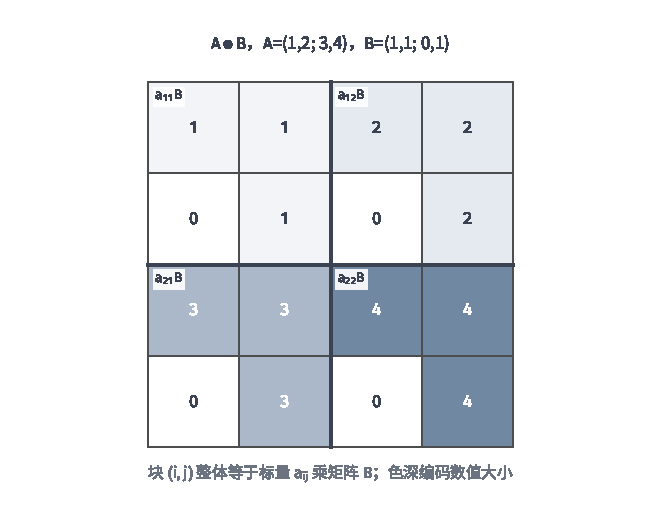
\includegraphics[width=112mm]{figures/00-shared/mathematical-preliminaries-upper/02-linear-spaces/matplotlib/ls-kronecker-block-structure/ls-kronecker-block-structure.pdf}
  \caption{Kronecker积的分块结构。上：$\bm A=\bigl(\begin{smallmatrix}1&2\\3&4\end{smallmatrix}\bigr)$、$\bm B=\bigl(\begin{smallmatrix}10&20\\30&40\end{smallmatrix}\bigr)$。下：$\bm A\otimes\bm B$是把$\bm A$的每个元素替换为该元素乘$\bm B$得到的$4\times4$分块矩阵，块边界用白线强调。数值由定义直接计算，是教学例。}
  \label{fig:ls-kronecker-block-structure}
\end{figure}

两个列向量按式~\eqref{eq:linear-algebra-kronecker-product}相乘，得到$mn$维长向量$(x_1\bm y^\top,\ldots,x_m\bm y^\top)^\top$，它正是把$m\times n$数组$\bm x\otimes\bm y$按行读出的结果。两种用法记录的是同一组数，只差一次按行读出，所以同一个记号$\otimes$不会引起混淆。例如$(1,2)^\top\otimes(3,-1)^\top=(3,-1,6,-2)^\top$，与示例~\ref{ex:ls-tensor-product-two-vectors}中的数组按行读出的结果相同。

\subsubsection{张量缩约}
\label{sec:ls-tensor-contraction}

张量积把槽位全部保留；缩约则沿指定的轴汇总。计算时选定一对或几对尺寸相同的轴，让每对轴共用同一个求和索引，逐项相乘后对这些索引求和；被求和的轴消失，其余轴保留，按原次序组成输出的形状。写出索引，就能检查哪些轴被消去、哪些轴应当保留，下面用两个例子说明这种检查。
\begin{example}[两种缩约的输出形状]
\label{ex:ls-contraction-shapes}
给定：（1）$\bm A\in\mathbb R^{m\times d\times r}$与$\bm B\in\mathbb R^{d\times n\times r}$；（2）$\bm X\in\mathbb R^{b\times\ell\times d}$与$\bm W\in\mathbb R^{d\times h}$。
计算：（1）让$\bm A$的第二轴与$\bm B$的第一轴共用索引$k$，两者的第三轴共用索引$s$，
\[
 c_{i,j}=\sum_{k=1}^d\sum_{s=1}^r a_{i,k,s}b_{k,j,s}.
\]
（2）让$\bm X$的最后一轴与$\bm W$的第一轴共用索引$k$，
\[
 z_{i,j,t}=\sum_{k=1}^d x_{i,j,k}w_{k,t}.
\]
结论：（1）同时消去$k$与$s$两对轴，保留$i,j$，输出为$m\times n$矩阵。（2）只消去$k$，保留$i,j,t$，输出形状为$b\times\ell\times h$：每个样本、每个位置上的$d$维特征都乘了同一个矩阵$\bm W$。
\end{example}
图~\ref{fig:ls-tensor-contraction}沿一对选中的轴求和并保留其余轴。
\begin{figure}[htbp]
  \centering
  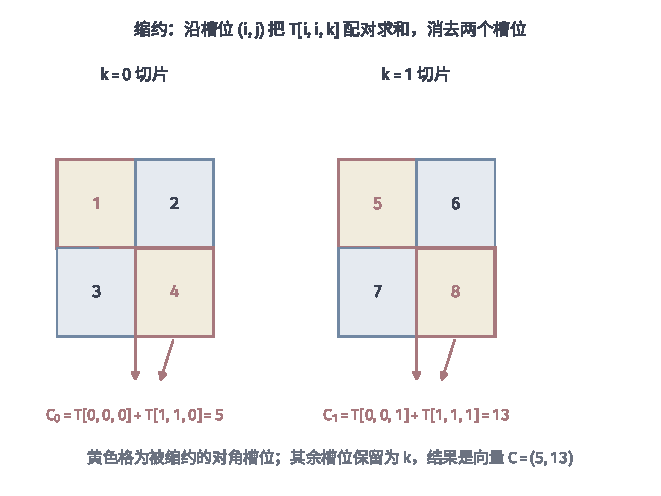
\includegraphics[width=112mm]{figures/00-shared/mathematical-preliminaries-upper/02-linear-spaces/matplotlib/ls-tensor-contraction/ls-tensor-contraction.pdf}
  \caption{张量缩约沿选中的一对轴求和、保留其余轴。左：二阶张量按行和列着色；选中列轴（虚线箭头）沿列求和，输出对每行汇总为一个值。右：缩约后得到$3$个输出，分别对应原矩阵三行的行和，颜色由红（小）经黄到蓝（大）。张量与数值均为解析教学例。}
  \label{fig:ls-tensor-contraction}
\end{figure}

前两节的几种运算都是缩约：
\begin{itemize}
 \item 内积$\sum_jx_jy_j$缩约两个向量唯一的一对轴，输出标量；
 \item 矩阵乘法$\sum_\ell a_{i,\ell}b_{\ell,j}$只消去左因子的列轴与右因子的行轴这一对；
 \item 迹$\sum_iA_{i,i}$把同一个矩阵的行轴与列轴对齐到同一索引后求和；
 \item Frobenius内积$\sum_{i,j}a_{i,j}b_{i,j}$同时缩约两对轴。
\end{itemize}

\subsection{张量运算的性质}
\label{sec:ls-tensor-operation-properties}

使用上一小节的运算时，须知道哪些操作可以撤销、括号怎样移动、Kronecker积怎样与普通矩阵乘法配合，以及缩约何时可以分开计算。本小节按运算整理，最后用一张表汇总各种“乘法”的形状条件。

\subsubsection{重排的性质}

\paragraph{可逆性}
目标形状与遍历顺序固定后，轴置换、形状重整与向量化都把一个数组一一对应到另一个数组，逆操作恢复原数组：转置再转置、按逆置换换回、按原顺序装回。例如$\operatorname{vec}$的逆操作把长度为$mn$的向量依次每$m$个一列装回$m\times n$矩阵。所以重排保留全部信息。

\paragraph{线性}
\[
 \operatorname{vec}(a\bm A+b\bm B)=a\operatorname{vec}(\bm A)+b\operatorname{vec}(\bm B),
\]
轴置换与形状重整同样满足这一性质：它们只搬动元素，逐项的加法与数乘搬到新位置后不变。

\paragraph{与矩阵乘法的关系}
转置与乘法有整齐的规则$(\bm A\bm B)^\top=\bm B^\top\bm A^\top$；一般的形状重整与乘法没有这样的关系。重整以后，矩阵每一行、每一列汇集的元素都变了，依赖行列结构的乘积、迹与行列式一般随之改变。下面的反例把示例~\ref{ex:ls-reshape-vs-transpose}中的$\bm R$误当作$\bm A^\top$使用。
\begin{example}[反例：重整不能代替转置]
\label{ex:ls-reshape-breaks-product}
给定：$\bm A=\left[\begin{smallmatrix}1&2&3\\4&5&6\end{smallmatrix}\right]$，以及按行重整得到的$\bm R=\left[\begin{smallmatrix}1&2\\3&4\\5&6\end{smallmatrix}\right]$。
计算：由示例~\ref{ex:ls-gram-product-symmetric}，$\bm A\bm A^\top=\left[\begin{smallmatrix}14&32\\32&77\end{smallmatrix}\right]$；而
\[
 \bm A\bm R=\begin{bmatrix}1+6+15&2+8+18\\4+15+30&8+20+36\end{bmatrix}=\begin{bmatrix}22&28\\49&64\end{bmatrix}.
\]
结论：$\bm R$与$\bm A^\top$形状相同、所含的数相同，两个乘积的迹却分别为$14+77=91$与$22+64=86$。
\end{example}
把存储格式的改变当成计算效果，是这里最常见的错误。

\subsubsection{张量积的性质}

\paragraph{对每个因子线性}
\[
 (a\bm x)\otimes\bm y=\bm x\otimes(a\bm y)=a(\bm x\otimes\bm y),\qquad
 (\bm x+\bm x')\otimes\bm y=\bm x\otimes\bm y+\bm x'\otimes\bm y,
\]
对第二个因子的加法同样分配。每个元素$x_iy_j$对$x_i$和$y_j$分别线性，逐项验证即得。

\paragraph{结合律}
\[
 (\bm x\otimes\bm y)\otimes\bm z=\bm x\otimes(\bm y\otimes\bm z),
\]
两边的$(i,j,k)$元素都是$x_iy_jz_k$。

\paragraph{交换槽位是转置}
\[
 \bm y\otimes\bm x=(\bm x\otimes\bm y)^\top,
\]
因为$\bm x\otimes\bm y$的$(i,j)$元素$x_iy_j$也是$\bm y\otimes\bm x$的$(j,i)$元素。所以一般$\bm x\otimes\bm y\neq\bm y\otimes\bm x$，两者相差一次轴置换。

\paragraph{Frobenius配对与范数分离}
\[
 \langle\bm x\otimes\bm y,\bm x'\otimes\bm y'\rangle_{\mathrm F}
 =\langle\bm x,\bm x'\rangle\langle\bm y,\bm y'\rangle,
 \qquad
 \lVert\bm x\otimes\bm y\rVert_{\mathrm F}=\lVert\bm x\rVert_2\,\lVert\bm y\rVert_2.
\]
第一式来自$\sum_{i,j}x_iy_jx'_iy'_j=(\sum_ix_ix'_i)(\sum_jy_jy'_j)$；第二式在第一式中取$\bm x'=\bm x$、$\bm y'=\bm y$后开平方。下面在示例~\ref{ex:ls-tensor-product-two-vectors}的数组上核对第二式。
\begin{example}[张量积范数的数值核对]
\label{ex:ls-tensor-product-norm-check}
给定：$\bm x=(1,2)^\top$，$\bm y=(3,-1)^\top$，$\bm x\otimes\bm y=\left(\begin{smallmatrix}3&-1\\6&-2\end{smallmatrix}\right)$。
计算：$\lVert\bm x\rVert_2=\sqrt5$，$\lVert\bm y\rVert_2=\sqrt{10}$；直接求Frobenius范数，
\[
 \lVert\bm x\otimes\bm y\rVert_{\mathrm F}=\sqrt{3^2+(-1)^2+6^2+(-2)^2}=\sqrt{50}.
\]
结论：$\sqrt5\cdot\sqrt{10}=\sqrt{50}=5\sqrt2$，两种算法一致。
\end{example}

\paragraph{与楔积的联系}
矩阵一节的楔积也可以由张量积经反对称化得到：$\bm x\wedge\bm y$对应$\bm x\otimes\bm y-\bm y\otimes\bm x$，交换$\bm x,\bm y$时它变号。这里只指出联系，楔积的规则不依赖张量积。

\subsubsection{Kronecker积的性质}
\label{sec:ls-kronecker-products}

\paragraph{分别作用于两个槽位}
\[
 (\bm A\otimes\bm B)(\bm x\otimes\bm y)=(\bm A\bm x)\otimes(\bm B\bm y).
\]
按分块乘法，左侧第$i$块为$\sum_jA_{i,j}\bm B(x_j\bm y)=(\sum_jA_{i,j}x_j)\bm B\bm y=(\bm A\bm x)_i\,\bm B\bm y$，正是右侧的第$i$块。第一个槽位只经过$\bm A$，第二个槽位只经过$\bm B$，两个作用并行而不串联；矩阵乘法则把前后两次作用串成一条链。

\paragraph{混合乘积}
当$\bm A\bm C$与$\bm B\bm D$分别有定义时，
\begin{equation}
 (\bm A\otimes\bm B)(\bm C\otimes\bm D)
 =(\bm A\bm C)\otimes(\bm B\bm D).
 \label{eq:matrix-analysis-kronecker-mixed-product}
\end{equation}
按分块乘法，左侧的块$(i,k)$为$\sum_j(A_{i,j}\bm B)(C_{j,k}\bm D)=(\sum_jA_{i,j}C_{j,k})\bm B\bm D=(\bm A\bm C)_{i,k}\bm B\bm D$，恰是右侧的块。上一条是$\bm C,\bm D$各只有一列的情形。

\paragraph{转置}
\[
 (\bm A\otimes\bm B)^\top=\bm A^\top\otimes\bm B^\top.
\]
分块矩阵转置时，块的位置交换，每块各自转置，所以第$(j,i)$块为$A_{i,j}\bm B^\top$，正是$\bm A^\top\otimes\bm B^\top$的第$(j,i)$块。

\paragraph{逆}
\[
 (\bm A\otimes\bm B)^{-1}=\bm A^{-1}\otimes\bm B^{-1}\qquad(\bm A,\bm B\text{都可逆}).
\]
由混合乘积，$(\bm A\otimes\bm B)(\bm A^{-1}\otimes\bm B^{-1})=(\bm A\bm A^{-1})\otimes(\bm B\bm B^{-1})=\bm I\otimes\bm I=\bm I$，另一侧同理。

\paragraph{迹}
\[
 \operatorname{tr}(\bm A\otimes\bm B)=\operatorname{tr}\bm A\,\operatorname{tr}\bm B\qquad(\bm A,\bm B\text{都是方阵}).
\]
只有对角块$A_{i,i}\bm B$的对角元落在主对角线上，所以迹为$\sum_iA_{i,i}\operatorname{tr}\bm B=\operatorname{tr}\bm A\,\operatorname{tr}\bm B$。

\paragraph{向量化恒等式}
对$\bm A\in\mathbb R^{p\times m}$、$\bm X\in\mathbb R^{m\times n}$、$\bm B\in\mathbb R^{n\times q}$，
\begin{equation}
 \operatorname{vec}(\bm A\bm X\bm B)
 =(\bm B^\top\otimes\bm A)\operatorname{vec}(\bm X).
 \label{eq:matrix-analysis-vec-kronecker}
\end{equation}
比较两侧输出的第$j$段（长度为$p$）。左侧是$\bm A\bm X\bm B$的第$j$列，$\bm A\bm X\bm B_{:,j}=\sum_kB_{k,j}\bm A\bm X_{:,k}$。右侧矩阵的第$j$块行为$(B_{1,j}\bm A,\ldots,B_{n,j}\bm A)$，与$\operatorname{vec}(\bm X)$的各段$\bm X_{:,1},\ldots,\bm X_{:,n}$相乘，也得到$\sum_kB_{k,j}\bm A\bm X_{:,k}$。逐元素写出，两侧$(i,j)$位置的元素都是$\sum_{\ell=1}^m\sum_{k=1}^n A_{i,\ell}X_{\ell,k}B_{k,j}$。

固定$\bm A,\bm B$后，这一恒等式把“两侧同时乘矩阵”写成对长向量$\operatorname{vec}(\bm X)$乘一张矩阵，从而把关于未知矩阵的方程化成普通线性方程组；第~\ref{chap:linear-equations-and-optimization}章求解矩阵方程时将用到它。

\subsubsection{缩约的性质}

\paragraph{线性}
固定配对数组后，缩约对被作用数组线性：把被作用数组换成$a\bm X+b\bm X'$，输出变为$a$倍与$b$倍两个输出之和。这是因为每个输出元素都是被作用数组元素以固定系数作的加权和。

\paragraph{求和次序可交换}
多对轴的缩约是有限和，结果与先消哪一对轴无关。例如示例~\ref{ex:ls-contraction-shapes}中的$c_{i,j}$可以先对$s$求和得到中间数组，再对$k$求和，也可以反过来。

\paragraph{简单张量系数可分离}
一次读取同时依赖三组向量$\bm x\in\mathbb R^m$、$\bm y\in\mathbb R^n$、$\bm z\in\mathbb R^p$时，若系数数组是简单张量$\bm a\otimes\bm b\otimes\bm c$，则
\begin{equation}
 \left\langle\bm a\otimes\bm b\otimes\bm c,
 \bm x\otimes\bm y\otimes\bm z\right\rangle_{\mathrm F}
 =(\bm a^\top\bm x)(\bm b^\top\bm y)(\bm c^\top\bm z),
 \label{eq:linear-algebra-rank-one-contraction}
\end{equation}
因为$\sum_{i,j,k}a_ib_jc_kx_iy_jz_k=(\sum_ia_ix_i)(\sum_jb_jy_j)(\sum_kc_kz_k)$：三重求和分离成三个内积的乘积，计算量从$mnp$项降到$m+n+p$项。下面用一组小数值核对。
\begin{example}[简单张量系数的分离计算]
\label{ex:ls-rank-one-contraction-check}
给定：$\bm a=(1,2)^\top$、$\bm b=(3,-1)^\top$、$\bm c=(2,1)^\top$，$\bm x=(2,1)^\top$、$\bm y=(1,1)^\top$、$\bm z=(1,-1)^\top$，这里$m=n=p=2$。
计算：三个内积依次为
\[
 \begin{gathered}
 \bm a^\top\bm x=1\cdot2+2\cdot1=4,\qquad
 \bm b^\top\bm y=3\cdot1+(-1)\cdot1=2,\\
 \bm c^\top\bm z=2\cdot1+1\cdot(-1)=1.
 \end{gathered}
\]
结论：由式~\eqref{eq:linear-algebra-rank-one-contraction}，读取等于$4\cdot2\cdot1=8$；直接展开三重求和要累加$2^3=8$项乘积，结果同样是$8$。
\end{example}

\paragraph{非线性操作不是缩约}
$\operatorname{softmax}$、逐元素非线性等操作不属于缩约。一个模型即使由缩约和这些操作交替组成，固定系数时每一步缩约的线性也不代表整体线性。

\subsubsection{各种乘积的形状}

本章出现了好几种“乘法”，它们的区别在于对索引做什么。表~\ref{tab:linear-algebra-products-and-shapes}汇总它们的形状条件与索引作用。

\begin{table*}[htbp]
 \centering\small
 \begin{tabularx}{\linewidth}{@{}lXX@{}}
  \toprule
  运算 & 形状条件与输出 & 索引作用\\
  \midrule
  $\langle\bm x,\bm y\rangle$ & 两个$n$维向量，输出标量 & 配对后汇总\\
  $\bm A\bm B$ & $(m\times n)(n\times p)\to m\times p$ & 汇总共同索引\\
  $\bm A\odot\bm B$ & 同为$m\times n$，输出仍为$m\times n$ & 同位置相乘，不求和\\
  $\bm x\otimes\bm y$ & $m$维与$n$维向量$\to m\times n$ & 保留两条轴，不求和\\
  $\bm A\otimes\bm B$ & $(m\times n)$与$(p\times q)\to(mp)\times(nq)$ & 保留两组成对索引\\
  缩约 & 被缩约的各对轴尺寸相同 & 消去指定轴，保留其余轴\\
  \bottomrule
 \end{tabularx}
 \caption{相乘符号对应不同操作。先检查消去哪些索引，再判断其线性性和输出含义。}
 \label{tab:linear-algebra-products-and-shapes}
\end{table*}
